\documentclass[11pt]{article}\usepackage[]{graphicx}\usepackage[]{color}
% maxwidth is the original width if it is less than linewidth
% otherwise use linewidth (to make sure the graphics do not exceed the margin)
\makeatletter
\def\maxwidth{ %
  \ifdim\Gin@nat@width>\linewidth
    \linewidth
  \else
    \Gin@nat@width
  \fi
}
\makeatother

\definecolor{fgcolor}{rgb}{0.345, 0.345, 0.345}
\newcommand{\hlnum}[1]{\textcolor[rgb]{0.686,0.059,0.569}{#1}}%
\newcommand{\hlstr}[1]{\textcolor[rgb]{0.192,0.494,0.8}{#1}}%
\newcommand{\hlcom}[1]{\textcolor[rgb]{0.678,0.584,0.686}{\textit{#1}}}%
\newcommand{\hlopt}[1]{\textcolor[rgb]{0,0,0}{#1}}%
\newcommand{\hlstd}[1]{\textcolor[rgb]{0.345,0.345,0.345}{#1}}%
\newcommand{\hlkwa}[1]{\textcolor[rgb]{0.161,0.373,0.58}{\textbf{#1}}}%
\newcommand{\hlkwb}[1]{\textcolor[rgb]{0.69,0.353,0.396}{#1}}%
\newcommand{\hlkwc}[1]{\textcolor[rgb]{0.333,0.667,0.333}{#1}}%
\newcommand{\hlkwd}[1]{\textcolor[rgb]{0.737,0.353,0.396}{\textbf{#1}}}%
\let\hlipl\hlkwb

\usepackage{framed}
\makeatletter
\newenvironment{kframe}{%
 \def\at@end@of@kframe{}%
 \ifinner\ifhmode%
  \def\at@end@of@kframe{\end{minipage}}%
  \begin{minipage}{\columnwidth}%
 \fi\fi%
 \def\FrameCommand##1{\hskip\@totalleftmargin \hskip-\fboxsep
 \colorbox{shadecolor}{##1}\hskip-\fboxsep
     % There is no \\@totalrightmargin, so:
     \hskip-\linewidth \hskip-\@totalleftmargin \hskip\columnwidth}%
 \MakeFramed {\advance\hsize-\width
   \@totalleftmargin\z@ \linewidth\hsize
   \@setminipage}}%
 {\par\unskip\endMakeFramed%
 \at@end@of@kframe}
\makeatother

\definecolor{shadecolor}{rgb}{.97, .97, .97}
\definecolor{messagecolor}{rgb}{0, 0, 0}
\definecolor{warningcolor}{rgb}{1, 0, 1}
\definecolor{errorcolor}{rgb}{1, 0, 0}
\newenvironment{knitrout}{}{} % an empty environment to be redefined in TeX

\usepackage{alltt}
%\usepackage[showframe]{geometry}
\usepackage[table]{xcolor}
\usepackage{caption}
\usepackage{lscape,verbatim,mathrsfs}
\usepackage{graphics,amsmath,pstricks}
\usepackage{amssymb,enumerate}
\usepackage{amsbsy,amsmath,amsthm,amsfonts, amssymb}
\usepackage{graphicx, rotate, array}
\usepackage{geometry,multirow}
\usepackage{color,soul}
\usepackage{float}
%\usepackage{hyperref}
\usepackage[authoryear,round]{natbib}
%\renewcommand{\baselinestretch}{1.9}
\usepackage{tcolorbox}
\renewcommand{\familydefault}{cmss}
\textwidth=6.65in \textheight=9.7in
\parskip=.025in
\parindent=0in
\oddsidemargin=-0.1in \evensidemargin=-.1in \headheight=-.6in
\footskip=0.5in \DeclareMathOperator*{\argmax}{argmax}
\DeclareMathOperator*{\argmin}{argmin}
\IfFileExists{upquote.sty}{\usepackage{upquote}}{}
\begin{document}


\title{SMART simulation - All Simulated (Real covs) Covariates}
\date{}

\maketitle













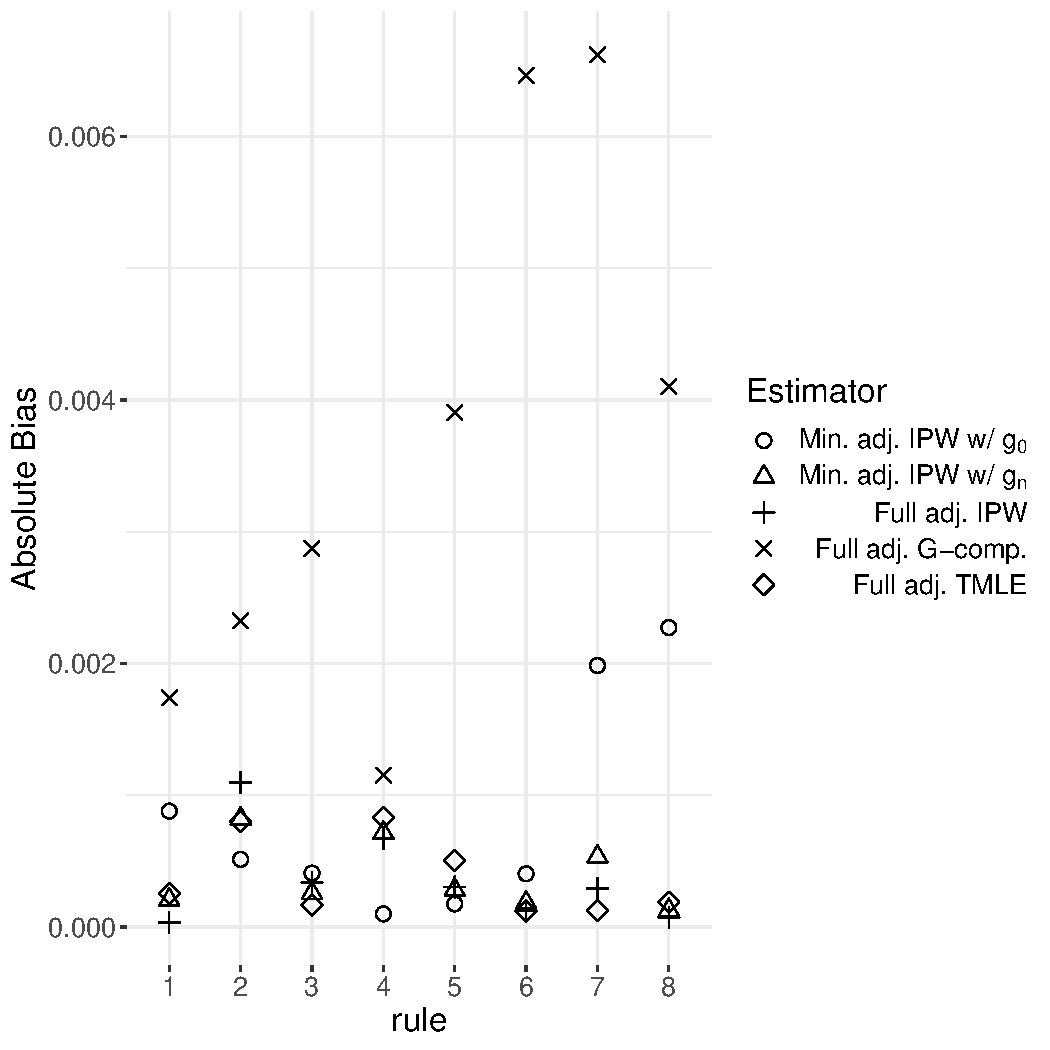
\includegraphics[width=\maxwidth]{figure/unnamed-chunk-3-1} 

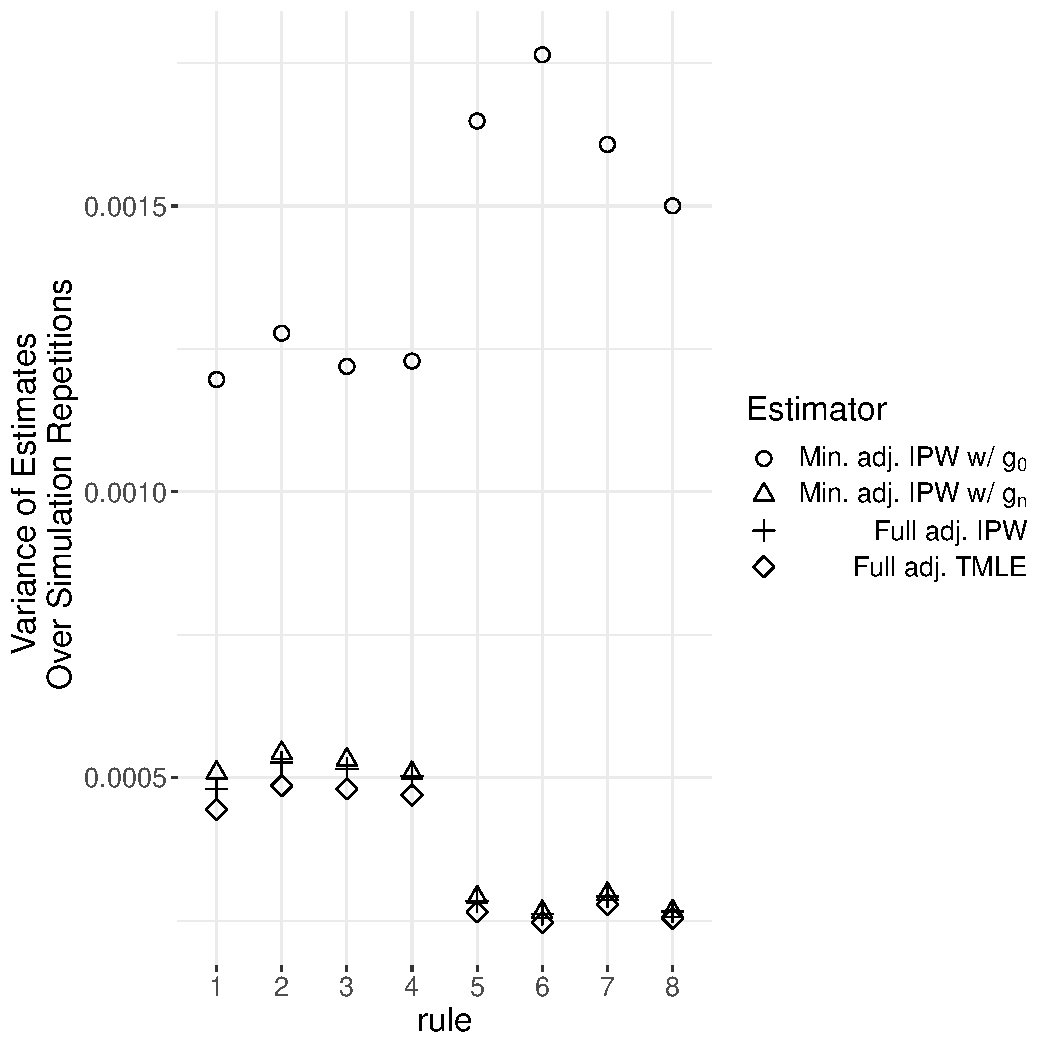
\includegraphics[width=\maxwidth]{figure/unnamed-chunk-3-2} 

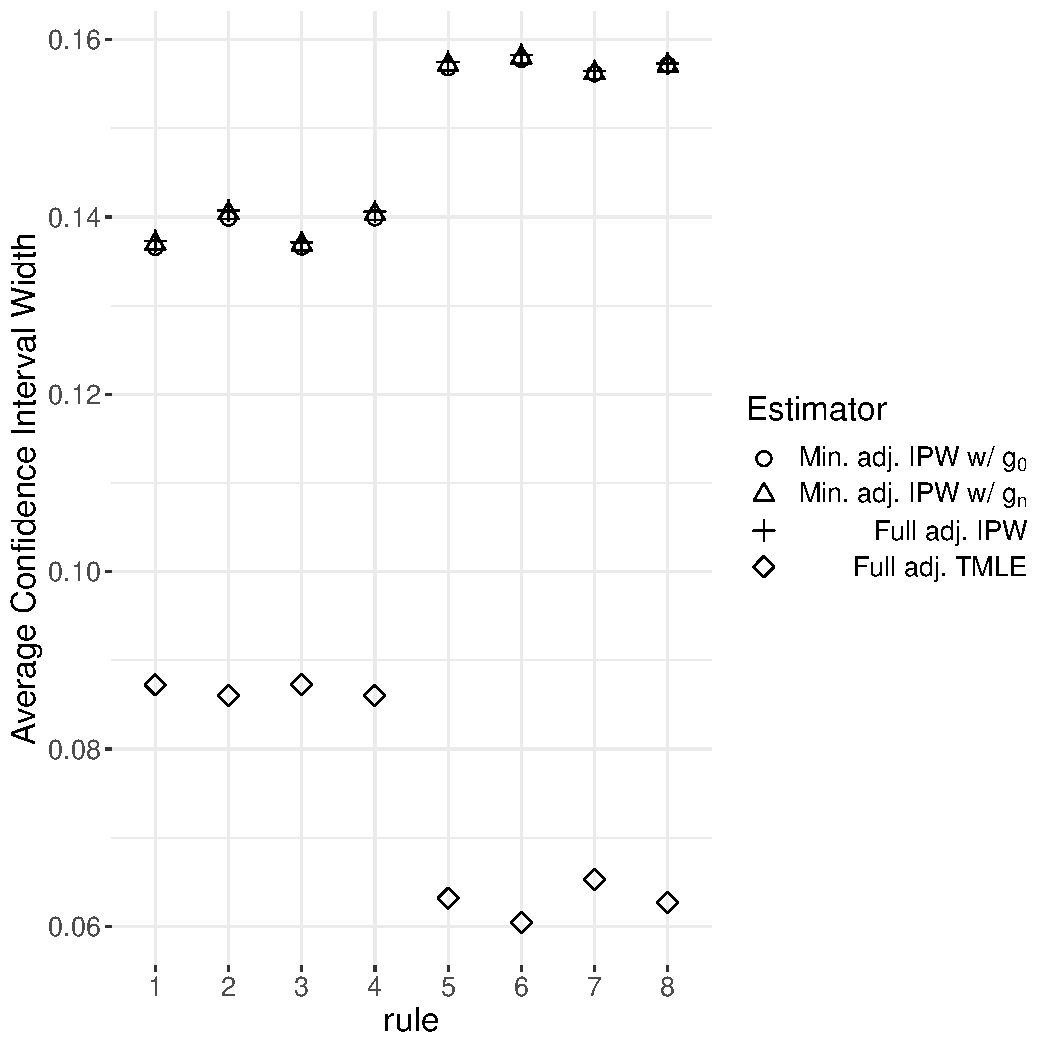
\includegraphics[width=\maxwidth]{figure/unnamed-chunk-3-3} 
pdf 
  2 



\begin{knitrout}
\definecolor{shadecolor}{rgb}{0.969, 0.969, 0.969}\color{fgcolor}\begin{kframe}
\begin{verbatim}
   Rule                Estimator         Bias         Var. C.I. Width
36    1 Min. adj. IPW (w/ $g_0$) 2.808647e-03 0.0023272797 0.18795782
37    1 Min. adj. IPW (w/ $g_n$) 1.500073e-03 0.0007990241 0.18919959
38    1           Full adj. IPTW 2.835077e-03 0.0007336945 0.19615706
39    1        Full adj. G-comp. 1.465137e-02           NA         NA
40    1           Full adj. TMLE 1.784771e-03 0.0004916176 0.08721119
66    2 Min. adj. IPW (w/ $g_0$) 1.693379e-03 0.0023222343 0.19026423
67    2 Min. adj. IPW (w/ $g_n$) 2.282251e-03 0.0007284508 0.19103391
68    2           Full adj. IPTW 2.974975e-03 0.0007297142 0.19826029
69    2        Full adj. G-comp. 1.140588e-03           NA         NA
70    2           Full adj. TMLE 1.744009e-03 0.0004777627 0.08613003
6     3 Min. adj. IPW (w/ $g_0$) 1.713476e-03 0.0022530074 0.18979943
7     3 Min. adj. IPW (w/ $g_n$) 1.058677e-04 0.0007524950 0.19122528
8     3           Full adj. IPTW 1.474570e-03 0.0006894648 0.19894015
9     3        Full adj. G-comp. 9.124380e-03           NA         NA
10    3           Full adj. TMLE 9.622125e-04 0.0005023252 0.08651203
46    4 Min. adj. IPW (w/ $g_0$) 5.885940e-04 0.0025915887 0.19204737
47    4 Min. adj. IPW (w/ $g_n$) 8.784304e-04 0.0007891027 0.19300241
48    4           Full adj. IPTW 1.604852e-03 0.0007588212 0.20097695
49    4        Full adj. G-comp. 6.584719e-03           NA         NA
50    4           Full adj. TMLE 8.417076e-04 0.0005070550 0.08522862
21    5 Min. adj. IPW (w/ $g_0$) 7.638404e-04 0.0024230440 0.18867341
22    5 Min. adj. IPW (w/ $g_n$) 4.058632e-04 0.0008336883 0.18959695
23    5           Full adj. IPTW 1.317958e-03 0.0007603245 0.19725593
24    5        Full adj. G-comp. 1.387736e-02           NA         NA
25    5           Full adj. TMLE 6.467377e-04 0.0005058092 0.08684067
56    6 Min. adj. IPW (w/ $g_0$) 3.511791e-04 0.0025760401 0.19095473
57    6 Min. adj. IPW (w/ $g_n$) 1.188289e-03 0.0007940230 0.19140422
58    6           Full adj. IPTW 1.458104e-03 0.0007931911 0.19932589
59    6        Full adj. G-comp. 2.012064e-03           NA         NA
60    6           Full adj. TMLE 5.942279e-04 0.0004980661 0.08569175
31    7 Min. adj. IPW (w/ $g_0$) 1.235687e-03 0.0014934521 0.14689361
32    7 Min. adj. IPW (w/ $g_n$) 7.028617e-04 0.0004616846 0.14755684
33    7           Full adj. IPTW 2.752914e-04 0.0004841683 0.15362450
34    7        Full adj. G-comp. 5.622333e-03           NA         NA
35    7           Full adj. TMLE 3.214255e-04 0.0003386089 0.07193991
1     8 Min. adj. IPW (w/ $g_0$) 4.888215e-04 0.0014263010 0.14881475
2     8 Min. adj. IPW (w/ $g_n$) 1.300263e-04 0.0004869303 0.14944036
3     8           Full adj. IPTW 7.830862e-04 0.0004905255 0.15666091
4     8        Full adj. G-comp. 1.117954e-02           NA         NA
5     8           Full adj. TMLE 5.113311e-04 0.0003495043 0.07056307
16    9 Min. adj. IPW (w/ $g_0$) 1.764982e-04 0.0014609520 0.14731154
17    9 Min. adj. IPW (w/ $g_n$) 4.069342e-04 0.0004811551 0.14834490
18    9           Full adj. IPTW 5.116463e-05 0.0004825169 0.15539801
19    9        Full adj. G-comp. 7.253513e-03           NA         NA
20    9           Full adj. TMLE 2.650669e-04 0.0003497118 0.07133550
41   10 Min. adj. IPW (w/ $g_0$) 9.081093e-04 0.0022854783 0.18850305
42   10 Min. adj. IPW (w/ $g_n$) 1.268820e-03 0.0008200322 0.18952080
43   10           Full adj. IPTW 1.441218e-04 0.0007524243 0.19705846
44   10        Full adj. G-comp. 1.307404e-02           NA         NA
45   10           Full adj. TMLE 1.050923e-03 0.0005114495 0.08712038
71   11 Min. adj. IPW (w/ $g_0$) 2.959054e-04 0.0023411699 0.19060601
72   11 Min. adj. IPW (w/ $g_n$) 1.037918e-03 0.0007513555 0.19172483
73   11           Full adj. IPTW 4.431420e-04 0.0007047480 0.19945092
74   11        Full adj. G-comp. 2.929682e-03           NA         NA
75   11           Full adj. TMLE 5.718015e-04 0.0004770814 0.08596317
11   12 Min. adj. IPW (w/ $g_0$) 2.494923e-04 0.0024160040 0.18990848
12   12 Min. adj. IPW (w/ $g_n$) 2.447960e-04 0.0007955413 0.19085638
13   12           Full adj. IPTW 2.035151e-03 0.0007358635 0.19834517
14   12        Full adj. G-comp. 7.401900e-03           NA         NA
15   12           Full adj. TMLE 1.739411e-04 0.0005179076 0.08656255
51   13 Min. adj. IPW (w/ $g_0$) 8.670839e-04 0.0025567189 0.19198296
52   13 Min. adj. IPW (w/ $g_n$) 4.810859e-04 0.0007584477 0.19303832
53   13           Full adj. IPTW 1.741519e-03 0.0007003532 0.20068694
54   13        Full adj. G-comp. 8.376234e-03           NA         NA
55   13           Full adj. TMLE 2.703804e-04 0.0004920886 0.08525414
26   14 Min. adj. IPW (w/ $g_0$) 5.098582e-04 0.0023360389 0.18877071
27   14 Min. adj. IPW (w/ $g_n$) 6.682052e-05 0.0008271942 0.18951678
28   14           Full adj. IPTW 1.180179e-03 0.0007781034 0.19696758
29   14        Full adj. G-comp. 1.218731e-02           NA         NA
30   14           Full adj. TMLE 9.949876e-04 0.0005218379 0.08692036
61   15 Min. adj. IPW (w/ $g_0$) 6.087234e-05 0.0023002492 0.19087527
62   15 Min. adj. IPW (w/ $g_n$) 1.226083e-04 0.0007480914 0.19171433
63   15           Full adj. IPTW 8.396858e-04 0.0006697974 0.19934604
64   15        Full adj. G-comp. 3.632964e-03           NA         NA
65   15           Full adj. TMLE 5.172186e-04 0.0004842798 0.08573242
   Ind. Cov. (%) Simult. Cov. (%)
36          93.6             92.7
37          99.8            100.0
38         100.0            100.0
39            NA               NA
40          94.9             92.6
66          94.7             92.7
67         100.0            100.0
68         100.0            100.0
69            NA               NA
70          95.0             92.6
6           95.6             92.7
7           99.8            100.0
8           99.9            100.0
9             NA               NA
10          95.3             92.6
46          94.2             92.7
47          99.8            100.0
48          99.9            100.0
49            NA               NA
50          94.1             92.6
21          94.1             92.7
22          99.8            100.0
23         100.0            100.0
24            NA               NA
25          94.5             92.6
56          94.2             92.7
57         100.0            100.0
58         100.0            100.0
59            NA               NA
60          94.6             92.6
31          94.7             92.7
32         100.0            100.0
33          99.9            100.0
34            NA               NA
35          93.5             92.6
1           94.8             92.7
2           99.9            100.0
3           99.9            100.0
4             NA               NA
5           94.4             92.6
16          95.1             92.7
17          99.7            100.0
18         100.0            100.0
19            NA               NA
20          94.6             92.6
41          95.5             92.7
42          99.8            100.0
43         100.0            100.0
44            NA               NA
45          93.7             92.6
71          94.7             92.7
72          99.8            100.0
73         100.0            100.0
74            NA               NA
75          94.3             92.6
11          94.9             92.7
12         100.0            100.0
13         100.0            100.0
14            NA               NA
15          94.6             92.6
51          93.9             92.7
52          99.8            100.0
53         100.0            100.0
54            NA               NA
55          94.3             92.6
26          95.1             92.7
27          99.9            100.0
28         100.0            100.0
29            NA               NA
30          94.1             92.6
61          94.3             92.7
62          99.9            100.0
63          99.9            100.0
64            NA               NA
65          94.9             92.6
\end{verbatim}
\end{kframe}
\end{knitrout}

Calcs
\begin{knitrout}
\definecolor{shadecolor}{rgb}{0.969, 0.969, 0.969}\color{fgcolor}\begin{kframe}
\begin{verbatim}
[1] 0.1140588 1.4651371
[1]   0.3833941 182.3887741
[1] 2.787059 5.195648
[1] 0.001269207 0.110130332
[1]  99.7 100.0
[1] 100 100
[1] 0.9535621 1.1168922
[1] 1.363474 5.195648
[1] 2.041893 2.358092
[1] 93.5 95.3
[1] 92.6 92.6
\end{verbatim}
\end{kframe}
\end{knitrout}











\end{document}
